
%% bare_conf.tex
%% V1.4b
%% 2015/08/26
%% by Michael Shell
%% See:
%% http://www.michaelshell.org/
%% for current contact information.
%%
%% This is a skeleton file demonstrating the use of IEEEtran.cls
%% (requires IEEEtran.cls version 1.8b or later) with an IEEE
%% conference paper.
%%
%% Support sites:
%% http://www.michaelshell.org/tex/ieeetran/
%% http://www.ctan.org/pkg/ieeetran
%% and
%% http://www.ieee.org/

%%*************************************************************************
%% Legal Notice:
%% This code is offered as-is without any warranty either expressed or
%% implied; without even the implied warranty of MERCHANTABILITY or
%% FITNESS FOR A PARTICULAR PURPOSE! 
%% User assumes all risk.
%% In no event shall the IEEE or any contributor to this code be liable for
%% any damages or losses, including, but not limited to, incidental,
%% consequential, or any other damages, resulting from the use or misuse
%% of any information contained here.
%%
%% All comments are the opinions of their respective authors and are not
%% necessarily endorsed by the IEEE.
%%
%% This work is distributed under the LaTeX Project Public License (LPPL)
%% ( http://www.latex-project.org/ ) version 1.3, and may be freely used,
%% distributed and modified. A copy of the LPPL, version 1.3, is included
%% in the base LaTeX documentation of all distributions of LaTeX released
%% 2003/12/01 or later.
%% Retain all contribution notices and credits.
%% ** Modified files should be clearly indicated as such, including  **
%% ** renaming them and changing author support contact information. **
%%*************************************************************************


% *** Authors should verify (and, if needed, correct) their LaTeX system  ***
% *** with the testflow diagnostic prior to trusting their LaTeX platform ***
% *** with production work. The IEEE's font choices and paper sizes can   ***
% *** trigger bugs that do not appear when using other class files.       ***                          ***
% The testflow support page is at:
% http://www.michaelshell.org/tex/testflow/



\documentclass[conference]{IEEEtran}
% Some Computer Society conferences also require the compsoc mode option,
% but others use the standard conference format.
%
% If IEEEtran.cls has not been installed into the LaTeX system files,
% manually specify the path to it like:
% \documentclass[conference]{../sty/IEEEtran}





% Some very useful LaTeX packages include:
% (uncomment the ones you want to load)


% *** MISC UTILITY PACKAGES ***
%
%\usepackage{ifpdf}
% Heiko Oberdiek's ifpdf.sty is very useful if you need conditional
% compilation based on whether the output is pdf or dvi.
% usage:
% \ifpdf
%   % pdf code
% \else
%   % dvi code
% \fi
% The latest version of ifpdf.sty can be obtained from:
% http://www.ctan.org/pkg/ifpdf
% Also, note that IEEEtran.cls V1.7 and later provides a builtin
% \ifCLASSINFOpdf conditional that works the same way.
% When switching from latex to pdflatex and vice-versa, the compiler may
% have to be run twice to clear warning/error messages.






% *** CITATION PACKAGES ***
%
%\usepackage{cite}
% cite.sty was written by Donald Arseneau
% V1.6 and later of IEEEtran pre-defines the format of the cite.sty package
% \cite{} output to follow that of the IEEE. Loading the cite package will
% result in citation numbers being automatically sorted and properly
% "compressed/ranged". e.g., [1], [9], [2], [7], [5], [6] without using
% cite.sty will become [1], [2], [5]--[7], [9] using cite.sty. cite.sty's
% \cite will automatically add leading space, if needed. Use cite.sty's
% noadjust option (cite.sty V3.8 and later) if you want to turn this off
% such as if a citation ever needs to be enclosed in parenthesis.
% cite.sty is already installed on most LaTeX systems. Be sure and use
% version 5.0 (2009-03-20) and later if using hyperref.sty.
% The latest version can be obtained at:
% http://www.ctan.org/pkg/cite
% The documentation is contained in the cite.sty file itself.


\usepackage{amsmath}
\usepackage{amsfonts}
\usepackage{amssymb}
\usepackage{amsthm}
\usepackage{algorithm2e}
\usepackage{listings}
\usepackage{xcolor}
\usepackage{tikz}
\usepackage{booktabs}
\usepackage{subfigure}
\usepackage[english]{babel}
\usepackage{blindtext}



% *** GRAPHICS RELATED PACKAGES ***
%
\ifCLASSINFOpdf
  % \usepackage[pdftex]{graphicx}
  % declare the path(s) where your graphic files are
  % \graphicspath{{../pdf/}{../jpeg/}}
  % and their extensions so you won't have to specify these with
  % every instance of \includegraphics
  % \DeclareGraphicsExtensions{.pdf,.jpeg,.png}
\else
  % or other class option (dvipsone, dvipdf, if not using dvips). graphicx
  % will default to the driver specified in the system graphics.cfg if no
  % driver is specified.
  % \usepackage[dvips]{graphicx}
  % declare the path(s) where your graphic files are
  % \graphicspath{{../eps/}}
  % and their extensions so you won't have to specify these with
  % every instance of \includegraphics
  % \DeclareGraphicsExtensions{.eps}
\fi
% graphicx was written by David Carlisle and Sebastian Rahtz. It is
% required if you want graphics, photos, etc. graphicx.sty is already
% installed on most LaTeX systems. The latest version and documentation
% can be obtained at: 
% http://www.ctan.org/pkg/graphicx
% Another good source of documentation is "Using Imported Graphics in
% LaTeX2e" by Keith Reckdahl which can be found at:
% http://www.ctan.org/pkg/epslatex
%
% latex, and pdflatex in dvi mode, support graphics in encapsulated
% postscript (.eps) format. pdflatex in pdf mode supports graphics
% in .pdf, .jpeg, .png and .mps (metapost) formats. Users should ensure
% that all non-photo figures use a vector format (.eps, .pdf, .mps) and
% not a bitmapped formats (.jpeg, .png). The IEEE frowns on bitmapped formats
% which can result in "jaggedy"/blurry rendering of lines and letters as
% well as large increases in file sizes.
%
% You can find documentation about the pdfTeX application at:
% http://www.tug.org/applications/pdftex





% *** MATH PACKAGES ***
%
%\usepackage{amsmath}
% A popular package from the American Mathematical Society that provides
% many useful and powerful commands for dealing with mathematics.
%
% Note that the amsmath package sets \interdisplaylinepenalty to 10000
% thus preventing page breaks from occurring within multiline equations. Use:
%\interdisplaylinepenalty=2500
% after loading amsmath to restore such page breaks as IEEEtran.cls normally
% does. amsmath.sty is already installed on most LaTeX systems. The latest
% version and documentation can be obtained at:
% http://www.ctan.org/pkg/amsmath





% *** SPECIALIZED LIST PACKAGES ***
%
%\usepackage{algorithmic}
% algorithmic.sty was written by Peter Williams and Rogerio Brito.
% This package provides an algorithmic environment fo describing algorithms.
% You can use the algorithmic environment in-text or within a figure
% environment to provide for a floating algorithm. Do NOT use the algorithm
% floating environment provided by algorithm.sty (by the same authors) or
% algorithm2e.sty (by Christophe Fiorio) as the IEEE does not use dedicated
% algorithm float types and packages that provide these will not provide
% correct IEEE style captions. The latest version and documentation of
% algorithmic.sty can be obtained at:
% http://www.ctan.org/pkg/algorithms
% Also of interest may be the (relatively newer and more customizable)
% algorithmicx.sty package by Szasz Janos:
% http://www.ctan.org/pkg/algorithmicx




% *** ALIGNMENT PACKAGES ***
%
%\usepackage{array}
% Frank Mittelbach's and David Carlisle's array.sty patches and improves
% the standard LaTeX2e array and tabular environments to provide better
% appearance and additional user controls. As the default LaTeX2e table
% generation code is lacking to the point of almost being broken with
% respect to the quality of the end results, all users are strongly
% advised to use an enhanced (at the very least that provided by array.sty)
% set of table tools. array.sty is already installed on most systems. The
% latest version and documentation can be obtained at:
% http://www.ctan.org/pkg/array


% IEEEtran contains the IEEEeqnarray family of commands that can be used to
% generate multiline equations as well as matrices, tables, etc., of high
% quality.




% *** SUBFIGURE PACKAGES ***
%\ifCLASSOPTIONcompsoc
%  \usepackage[caption=false,font=normalsize,labelfont=sf,textfont=sf]{subfig}
%\else
%  \usepackage[caption=false,font=footnotesize]{subfig}
%\fi
% subfig.sty, written by Steven Douglas Cochran, is the modern replacement
% for subfigure.sty, the latter of which is no longer maintained and is
% incompatible with some LaTeX packages including fixltx2e. However,
% subfig.sty requires and automatically loads Axel Sommerfeldt's caption.sty
% which will override IEEEtran.cls' handling of captions and this will result
% in non-IEEE style figure/table captions. To prevent this problem, be sure
% and invoke subfig.sty's "caption=false" package option (available since
% subfig.sty version 1.3, 2005/06/28) as this is will preserve IEEEtran.cls
% handling of captions.
% Note that the Computer Society format requires a larger sans serif font
% than the serif footnote size font used in traditional IEEE formatting
% and thus the need to invoke different subfig.sty package options depending
% on whether compsoc mode has been enabled.
%
% The latest version and documentation of subfig.sty can be obtained at:
% http://www.ctan.org/pkg/subfig




% *** FLOAT PACKAGES ***
%
%\usepackage{fixltx2e}
% fixltx2e, the successor to the earlier fix2col.sty, was written by
% Frank Mittelbach and David Carlisle. This package corrects a few problems
% in the LaTeX2e kernel, the most notable of which is that in current
% LaTeX2e releases, the ordering of single and double column floats is not
% guaranteed to be preserved. Thus, an unpatched LaTeX2e can allow a
% single column figure to be placed prior to an earlier double column
% figure.
% Be aware that LaTeX2e kernels dated 2015 and later have fixltx2e.sty's
% corrections already built into the system in which case a warning will
% be issued if an attempt is made to load fixltx2e.sty as it is no longer
% needed.
% The latest version and documentation can be found at:
% http://www.ctan.org/pkg/fixltx2e


%\usepackage{stfloats}
% stfloats.sty was written by Sigitas Tolusis. This package gives LaTeX2e
% the ability to do double column floats at the bottom of the page as well
% as the top. (e.g., "\begin{figure*}[!b]" is not normally possible in
% LaTeX2e). It also provides a command:
%\fnbelowfloat
% to enable the placement of footnotes below bottom floats (the standard
% LaTeX2e kernel puts them above bottom floats). This is an invasive package
% which rewrites many portions of the LaTeX2e float routines. It may not work
% with other packages that modify the LaTeX2e float routines. The latest
% version and documentation can be obtained at:
% http://www.ctan.org/pkg/stfloats
% Do not use the stfloats baselinefloat ability as the IEEE does not allow
% \baselineskip to stretch. Authors submitting work to the IEEE should note
% that the IEEE rarely uses double column equations and that authors should try
% to avoid such use. Do not be tempted to use the cuted.sty or midfloat.sty
% packages (also by Sigitas Tolusis) as the IEEE does not format its papers in
% such ways.
% Do not attempt to use stfloats with fixltx2e as they are incompatible.
% Instead, use Morten Hogholm'a dblfloatfix which combines the features
% of both fixltx2e and stfloats:
%
% \usepackage{dblfloatfix}
% The latest version can be found at:
% http://www.ctan.org/pkg/dblfloatfix




% *** PDF, URL AND HYPERLINK PACKAGES ***
%
%\usepackage{url}
% url.sty was written by Donald Arseneau. It provides better support for
% handling and breaking URLs. url.sty is already installed on most LaTeX
% systems. The latest version and documentation can be obtained at:
% http://www.ctan.org/pkg/url
% Basically, \url{my_url_here}.




% *** Do not adjust lengths that control margins, column widths, etc. ***
% *** Do not use packages that alter fonts (such as pslatex).         ***
% There should be no need to do such things with IEEEtran.cls V1.6 and later.
% (Unless specifically asked to do so by the journal or conference you plan
% to submit to, of course. )


% correct bad hyphenation here
\hyphenation{op-tical net-works semi-conduc-tor}


\begin{document}
%
% paper title
% Titles are generally capitalized except for words such as a, an, and, as,
% at, but, by, for, in, nor, of, on, or, the, to and up, which are usually
% not capitalized unless they are the first or last word of the title.
% Linebreaks \\ can be used within to get better formatting as desired.
% Do not put math or special symbols in the title.
\title{Industrial Internet of Things for Resource\\ Constraint Devices}


% author names and affiliations
% use a multiple column layout for up to three different
% affiliations
\author{\IEEEauthorblockN{Viraj Kulkarni}
\IEEEauthorblockA{Technical University of Darmstadt\\
Email: viraj.kulkarni@stud.tu-darmstadt.de}
\and
\IEEEauthorblockN{David Abuladze}
\IEEEauthorblockA{Technical University of Darmstadt\\
Email: david.abuladze@stud.tu-darmstadt.de}}

% conference papers do not typically use \thanks and this command
% is locked out in conference mode. If really needed, such as for
% the acknowledgment of grants, issue a \IEEEoverridecommandlockouts
% after \documentclass

% for over three affiliations, or if they all won't fit within the width
% of the page, use this alternative format:
% 
%\author{\IEEEauthorblockN{Michael Shell\IEEEauthorrefmark{1},
%Homer Simpson\IEEEauthorrefmark{2},
%James Kirk\IEEEauthorrefmark{3}, 
%Montgomery Scott\IEEEauthorrefmark{3} and
%Eldon Tyrell\IEEEauthorrefmark{4}}
%\IEEEauthorblockA{\IEEEauthorrefmark{1}School of Electrical and Computer Engineering\\
%Georgia Institute of Technology,
%Atlanta, Georgia 30332--0250\\ Email: see http://www.michaelshell.org/contact.html}
%\IEEEauthorblockA{\IEEEauthorrefmark{2}Twentieth Century Fox, Springfield, USA\\
%Email: homer@thesimpsons.com}
%\IEEEauthorblockA{\IEEEauthorrefmark{3}Starfleet Academy, San Francisco, California 96678-2391\\
%Telephone: (800) 555--1212, Fax: (888) 555--1212}
%\IEEEauthorblockA{\IEEEauthorrefmark{4}Tyrell Inc., 123 Replicant Street, Los Angeles, California 90210--4321}}




% use for special paper notices
%\IEEEspecialpapernotice{(Invited Paper)}




% make the title area
\maketitle

% As a general rule, do not put math, special symbols or citations
% in the abstract
\begin{abstract}
The abstract goes here.
\end{abstract}

% no keywords




% For peer review papers, you can put extra information on the cover
% page as needed:
% \ifCLASSOPTIONpeerreview
% \begin{center} \bfseries EDICS Category: 3-BBND \end{center}
% \fi
%
% For peerreview papers, this IEEEtran command inserts a page break and
% creates the second title. It will be ignored for other modes.
\IEEEpeerreviewmaketitle



\section{Introduction}
% no \IEEEPARstart
This demo file is intended to serve as a ``starter file''
for IEEE conference papers produced under \LaTeX\ using
IEEEtran.cls version 1.8b and later.
% You must have at least 2 lines in the paragraph with the drop letter
% (should never be an issue)
I wish you the best of success.

\hfill mds
 
\hfill August 26, 2015


\subsection{Reducing the network footprint}
Dürkop et al (2012) have identified that the memory footprint for current OPC UA was too high for small devices \cite{durkop2012service}. In this work \cite{durkop2012service} two Service Oriented Architectures (SOA) for autoconfiguration of real-time ethernet systems have been introduced. The first Architecture is Device Profile for Web Service (DPWS) and the second is OPC UA. In addition to these SOAs, memory footprint for OPC UA implementation has been discussed. It has been emphasized, that significantly less program and data memory was needed for OPC UA, and number of code lines was less than a half of the DPWS. For both DPWS and OPC UA servers the Tiger Profinet Solution (TPS-1) has been chosen. It was extended the firmware by OPC UA stack using binary encoding. The OPC UA server was implemented on the Nano Embedded Device Server profiles. The binary transport profile was assigned, and the authentication using certificates have been used for the support. Dürkop et al (2012) have concluded that OPC UA requires significantly less hardware resources. Authors have emphasized that OPC UA server was developed from scratch in order to achieve small memory footprint for embedded devices. Further, in the article \cite{shrestha2013optimized} it has been discussed how to minimize the OPC UA network footprint in order to fit Bluetooth Low energy (BLE) frame. In paper \cite{imtiaz2013scalability} authors have implemented TCP-1 with real-time Ethernet interfaces, but the problem with devices with different transport protocol technologies, such as BLE, CAN bus, has appeared. The cause of this problem is low payload size of these protocol technologies. That is the reason why the authors \cite{shrestha2013optimized} have suggested to optimize OPC UA information model to suite it for BLE and CAN bus. In their article, authors have proposed to optimize the size of OPC UA in ReadResponse fields.
\begin{figure}[ht]
\centering
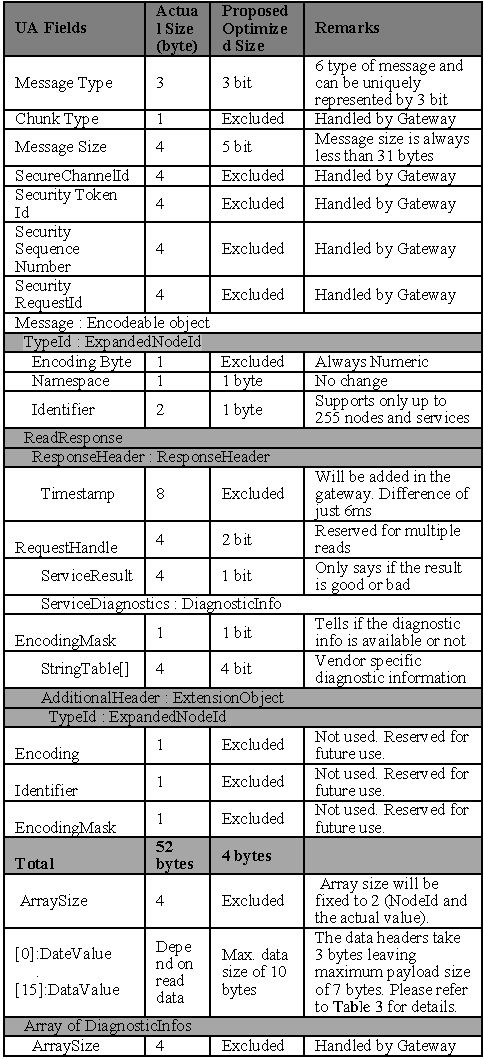
\includegraphics[width=0.78\linewidth]{Figures/optimize}\quad
\caption[Subfigure optimize]{\label{f:optimize}
Message size dependence on the used encoding from \cite{middleware2014optimizing}, p.1574}
\end{figure} 
 OPC UA Transport Profile (OOTP) with TCP/IP protocol has been implemented. As a result, OPC UA optimized header uses only 7 bytes and there are 7 bytes left for payload. This article has presented the possibility to integrate the OPC UA network footprint to the different small devices.



\subsection{Efficient OPC UA encoding}
The next improvement area for embedded devices is a possibility to encode data. It allows transferring data for devices with limited access memory \cite{efficient2016binaryencoding}. Reduced bandwidth becomes a very important aspect, because it is increasing use of “smart” field devices in industrial networks and there is also semantic integration for device layers \cite{efficient2016binaryencoding}. Article \cite{middleware2014optimizing} integrate different performance optimization techniques into the OPC UA. This include asynchronous communication and different encoding possibilities). OPC UA has been working in the IEC 61850-OPC UA mapping system (IEC 61850 is communication protocol which is international defined). Proposed possibilities have been analyzed in simulation environment. OPC UA communication is based on XML-based web service. To reduce message size two encoding technologies where discussed, such as EXI and Binary. There are several articles which highlight this technologies \cite{efficient2016binaryencoding} \cite{middleware2014optimizing}.First \cite{middleware2014optimizing} article discuses both XML Interchange (EXI) and Binary encoding and second only binary encoding. The EXI is a design for high performance parsing, which contains main benefits of both the XML and UA Binary - the binary encoding is the most efficient and it has less message size, but EXI is web technology and have good tool support \cite{middleware2014optimizing}.

\begin{figure}[ht]
\centering
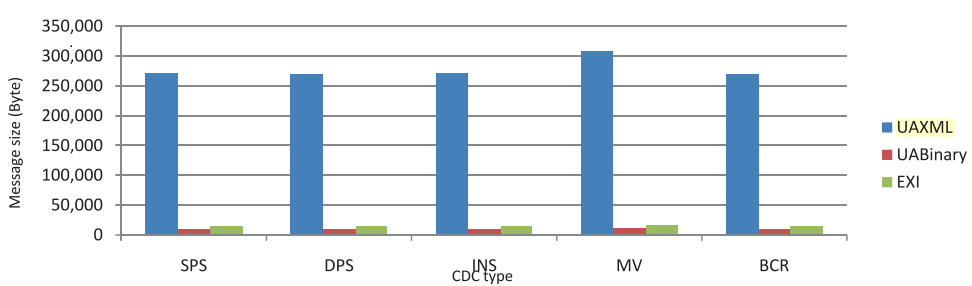
\includegraphics[width=1\linewidth]{Figures/encoding}\quad
\caption[Subfigure example]{\label{f:encoding}Message size dependence on the used encoding from \cite{middleware2014optimizing}, p.1574}
\end{figure}
 

In Figure 1 shows, that UA binary and EXI encoding have significant reduced message size compared to the XML. But between EXI and Binary is not much difference. The next article \cite{efficient2016binaryencoding} describes the binary encoding for limited memory devices. Main focus was on single-chip microcomputing platforms. Goal was to reduce bandwidth to (116 kB for Namespace 0). It was clarified that, if we want to improve bandwidth, it is possible only if data is compressed as a service\cite{efficient2016binaryencoding}. Parsing XML data are problematic and it is necesary to parse data in memory to access it efficiently. That was the reason why authors presented  OPC UA hardware server IP Core to overcome the limitation. To use this technology binary encoding was created. As a result binary encoding was suitable for small devices such as 8 bit Electrically Erasable Programmable Read-Only Memory (EEPROM) and Flash memory products. String compression demonstrated that the memory requirements have reduced from 197 kb to 116 kb, which corresponds to the 56\% of improvement\cite{efficient2016binaryencoding}.



\subsection{Efficient address space}
This problem is addressed in the paper “Efficient address space generation for an OPC UA Server” by Girbea et al (2011) [1]. Address space improvement is a very important aspect to get the speedup for development and maintenance time. In order to understand the structure of OPC UA Serve, the startup procedure has been discussed. OPC UA Server startup consists of multiple steps, as presented on the Figure~\ref{f:Steps}. 

\begin{figure}[ht]
\centering
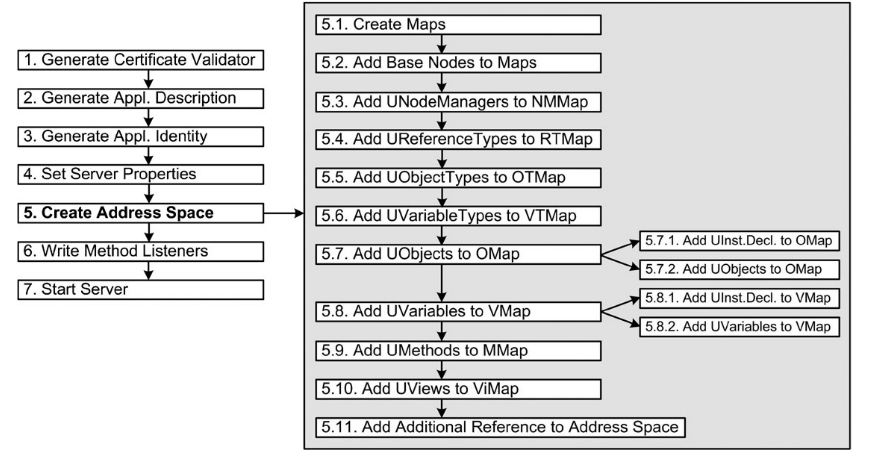
\includegraphics[width=1\linewidth]{Figures/Steps}\quad
\caption{\label{f:Steps}Wide single column figure in a twocolumn document.}
\end{figure}

On the left-hand side of the Figure~\ref{f:Steps} there are main steps to be programmed. The list of the actions for the address space generation are presented on the right-hand side of the Figure~\ref{f:Steps} [1]. The authors claim that the main units of address space are nodes and connected references. The base nodes are abstract and all the other nodes are subparts of base nodes, such as variable, variabletype, object objecttype, data view and method. There are 4 algorithms have been implemented, created for type nodes, for methods, for view and for object. There can be some similarities in these 4 algorithms. Nevertheless, the details description of each algorithm is not relevant for this seminar paper. The first algorithm uses referencetype hierarchy and have several similar properties with objecttypes and variabletypes. The second algorithm uses object nodes hierarchy and is similar to the variable nodes. The third algorithm is based on method nodes. This algorithm adds the nodes in success groups. The fourth algorithm generates the view nodes hierarchy. Algorithm 5 is simple and it reads the source, gets target node and reference and after that adds reference to address space\cite{addressspace2012efficient}. 

\begin{figure}[ht]
\centering
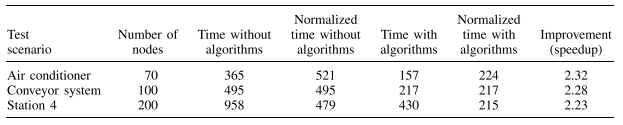
\includegraphics[width= 1\linewidth]{Figures/Table1new}\quad
\caption[Subfigure example]{\label{f:Table1new} Improvement of development time from \cite{addressspace2012efficient} p. 555.}

\end{figure}

\begin{figure}[ht]
\centering
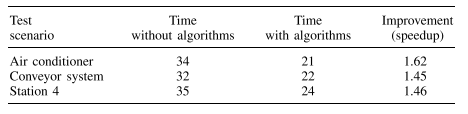
\includegraphics[width= 1\linewidth]{Figures/Table2new}\quad
\caption[Subfigure example]{\label{f:Table2new} Improvement of maintenance time  from \cite{addressspace2012efficient} p. 556.}
\end{figure}

Figure 3 shows that the main advantage of the presented algorithms is reduced development time. Speedup was around 2.2-2.3

Figure 4 shows that  maintenance time speedup was 1.4-1.6 

\begin{figure}[ht]
\centering
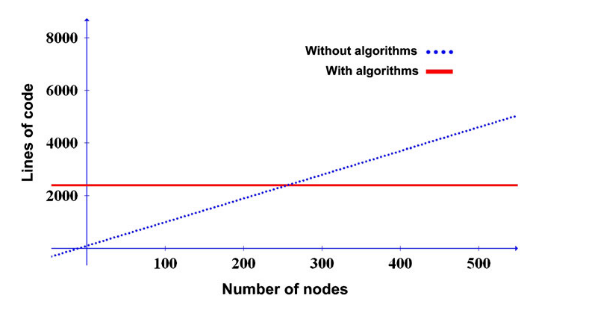
\includegraphics[width=1\linewidth]{Figures/NodeAlgorithm}\quad
\caption[Subfigure example]{\label{f:NodeAlgorithm}From \cite{addressspace2012efficient} p. 555 Lines of code used to generate the address space.}
\end{figure}

Figurem 8 shows that line of code is constant and independent of node number. This means that the more nodes the more efficient will be the algorithm. 

results of implemented algorithms shows significant improvement in comparison to the address space generaion without the algorithms, presented above. The nodes can also be modified by UA Server Admin in online or offline mode and by client in online mode.

\subsection{Security}
One of the main parameters of the OPC UA specification that has a significant impact on performance of the resource constrained devices is security. As stated in the part 7 of the OPC UA specifications, OPC UA provides three security profiles: Basic128Rsa15, Basic256 and None. Since OPC UA is used at different levels of automation in disparate applications within the same environment, a good trade off between the security and performance should be reached. This can bne done by taking into consideration, the level at which OPC UA is implemented. For example, At the very high level, where the device resources are abundant and where security might be more important than the performance, the profile which provides the highest amount of security should be used. Where as at very low levels, like in embedded devices where the device resources are very scarce, but security might not be as important as the performance, a weaker security profile which favors performance should be used.

Based on this premise, Olli Post, Jari Sepp\"al\"a and Hannu Koivisto have measured the performance of resource constrained devices in the paper "The performance of OPC UA security model at field device level". The findings of the evaluation are as follows. \cite{post2009performance}

For the evaluation of the performance in terms of efficient data transfer, all the three security profiles of the OPC UA specification namely None, Basic256 and Basic128Rsa15 as well as IPSec AH were compared. The evaluation was done to asses the delay caused by security measures with three packet sizes 1024 bytes, 10 240 bytes and 10 400 bytes.

IPSec is a network layer protocol that guarantees data confidentiality and integrity, origin identification and prevent replay attacks (Douligeriset al., 2007)\cite{post2009performance}

\begin{figure}[ht]
\centering
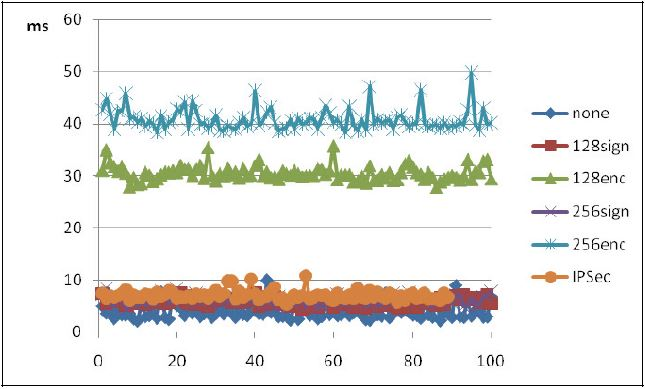
\includegraphics[height=50mm]{Figures/security_fig2}\quad
\caption[Subfigure example]{\label{f:security_fig2}Comparison between different OPC UA security profiles\\ with 102400 bytes \cite{post2009performance}}
\end{figure}

The first evaluation was done on 10 240 bytes which is represented in the figure~\ref{f:security_fig2}. The figure shows the delay caused by none, 128signed, 128encrypted, 256signed, 256encrypted and IPSec profiles. It can be seen in the figure that there is a tremendous delay when the data was encrypted in cases of 128encrypted and 265encrypted as opposed to the security profile None. Hence based on the evaluation, it is safe to say that in field or embedded devices which are strapped for resources and where confidentiality of the data is not a strict requirement, encryption adds a significant delay and is not an optimal solution for efficient data transfer. 

\begin{figure}[ht]
\centering
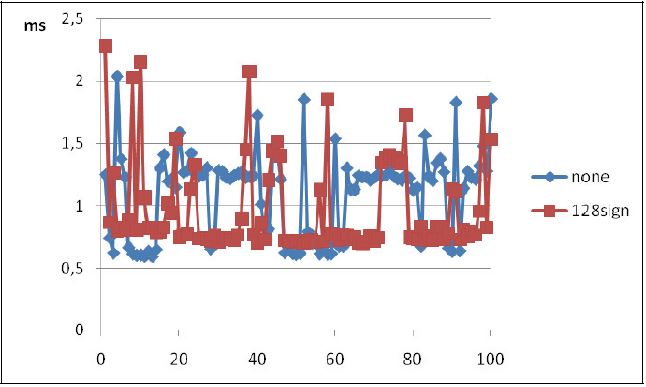
\includegraphics[height=50mm]{Figures/security_fig3}\quad
\caption[Subfigure example]{\label{f:security_fig3}Delay caused in a data size of 1024 bytes \cite{post2009performance}}
\end{figure}

\begin{figure}[ht]
\centering
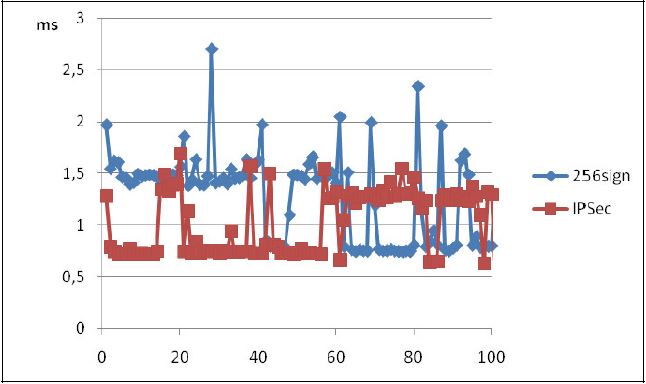
\includegraphics[height=50mm]{Figures/security_fig4}\quad
\caption[Subfigure example]{\label{f:security_fig4}Delay caused in a data size of 1024 bytes \cite{post2009performance}}
\end{figure}

The next performance measurements were done with a small data size of 1024 Bytes. The figures~\ref{f:security_fig3} and ~\ref{f:security_fig4} show the delay caused in sending packets with 1024 bytes. The figure~\ref{f:security_fig3} and ~\ref{f:security_fig4} depict the comparison between the profiles None, Basic128 and the Basic256 , IPSec AH. It can be inferred from the diagrams that authentication does not have a big impact in terms of delay in small packets of 1024 bytes.	 	 


\subsubsection{Subsubsection Heading Here}
Subsubsection text here.

\subsection{Scalability}
OPC UA is used to enable Internet of Things for industrial automation applications which provides powerful information representation that is exchangeable through inter operable services. The scalability of OPC UA refers to the ability of the hardware devices at different levels in the same environment to implement OPC UA efficiently. The problem with most of the current implementations of OPC UA is that they come with a lot of features which might not be needed by a hardware device at a certain level. Since each hardware device does not have the capability to implement every feature of OPC UA, the implementation  of all the features including the ones which are not used by the device puts unnecessary strain on the device in terms of memory, network overhead etc. 
Some off the shelf implementations of OPC UA take as much as 10MB of memory. \cite{6622935} The memory required by the OPC UA implementation is directly proportional to the number of features implemented and the complexity of those features. But some devices in the environment may have as less as a few kilo bytes of memory. Hence off the shelf implementation of OPC UA is not suitable for such devices. New stripped down implementations need to be tested for such resource limited devices. 

The paper "Scalability of OPC-UA down to the chip level enables Internet of Things" by Jahanzaib Imtiaz and Jürgen Jasperneite investigates one such implementation of OPC UA for resource limited devices based on the "Nano Embedded Device Server Profile" of the OPC foundation. This profile servers two purposes. First is to reduce the complexity of the implementation and the second is to minimize the memory footprint enabling it to be used on smaller devices.------------cite the paper -----------


\begin{figure}[ht]
\centering
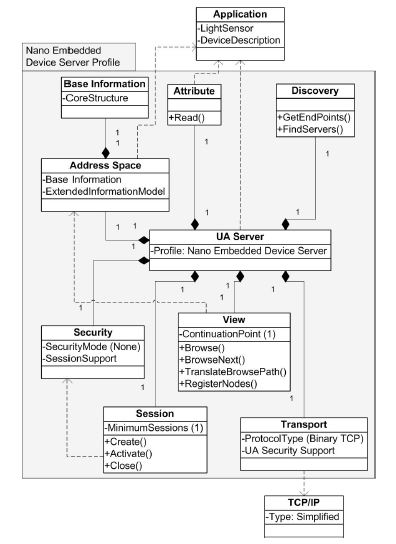
\includegraphics[height=125mm]{Figures/nano_embeddedSP}\quad
\caption[Subfigure example]{\label{f:nano_embeddedSP}Components of Nano Embedded Device Server profile}
\end{figure}


\subsubsection{Nano Embedded Device Server Profile}
This is a profile which encapsulates all the essential features of the OPC UA and describes a bare minimal OPC UA server functionality for small constrained devices. It uses the TCP binary protocol as the transport profile.
The components of this profile are:

\begin{itemize}
\item An Address Space component that describes the information model of the application which is exposed to the external environment. ----- cite -----

\item The Security component deals with the authentication and encryption aspects. In smaller devices, stringent security is not emphasized. This component provides security compliant with the "None" security profile of OPC UA.  ------ cite-----

\item The Session component is responsible for establishing a single secure session between the client and the server at any given time. ------ cite-----

\item The transport component implements a binary transport mechanism on top of TCP\textbackslash IP.

\item The Discovery component implements the discovery service without registering to the external discovery server. It answers the self discovery queries from the external clients. ------------cite-----

\item The View component traverses through the information model and browses the application specific address space.

\item The Attribute component is responsible for reading and writing of specific attributes of an object in the address space.
\end{itemize}

In the paper, the authors have conducted a simple case study of implementing this nano server profile to test the effectiveness of it. The case study consists of sue case of IoT in industrial automation domain. ---------- cite--------------
Upon implementation of this profile, it was found that OPC UA can be successfully scaled down to the small memory constrained devices while still retaining all the main features of the OPC UA.
It was found that the OPC UA server with basic set of services can be implemented in as less as 10 KB of the memory excluding the TCP\textbackslash IP.
Also, using this profile has simplified the software integration  in most of the smallest devices in the internet of things. Thus, using this profile has demonstrated the high saclability of OPC UA enabling the efficient use of the OPC UA specification at any level of the automation pyramid.

% An example of a floating figure using the graphicx package.
% Note that \label must occur AFTER (or within) \caption.
% For figures, \caption should occur after the \includegraphics.
% Note that IEEEtran v1.7 and later has special internal code that
% is designed to preserve the operation of \label within \caption
% even when the captionsoff option is in effect. However, because
% of issues like this, it may be the safest practice to put all your
% \label just after \caption rather than within \caption{}.
%
% Reminder: the "draftcls" or "draftclsnofoot", not "draft", class
% option should be used if it is desired that the figures are to be
% displayed while in draft mode.
%
%\begin{figure}[!t]
%\centering
%\includegraphics[width=2.5in]{myfigure}
% where an .eps filename suffix will be assumed under latex, 
% and a .pdf suffix will be assumed for pdflatex; or what has been declared
% via \DeclareGraphicsExtensions.
%\caption{Simulation results for the network.}
%\label{fig_sim}
%\end{figure}

% Note that the IEEE typically puts floats only at the top, even when this
% results in a large percentage of a column being occupied by floats.


% An example of a double column floating figure using two subfigures.
% (The subfig.sty package must be loaded for this to work.)
% The subfigure \label commands are set within each subfloat command,
% and the \label for the overall figure must come after \caption.
% \hfil is used as a separator to get equal spacing.
% Watch out that the combined width of all the subfigures on a 
% line do not exceed the text width or a line break will occur.
%
%\begin{figure*}[!t]
%\centering
%\subfloat[Case I]{\includegraphics[width=2.5in]{box}%
%\label{fig_first_case}}
%\hfil
%\subfloat[Case II]{\includegraphics[width=2.5in]{box}%
%\label{fig_second_case}}
%\caption{Simulation results for the network.}
%\label{fig_sim}
%\end{figure*}
%
% Note that often IEEE papers with subfigures do not employ subfigure
% captions (using the optional argument to \subfloat[]), but instead will
% reference/describe all of them (a), (b), etc., within the main caption.
% Be aware that for subfig.sty to generate the (a), (b), etc., subfigure
% labels, the optional argument to \subfloat must be present. If a
% subcaption is not desired, just leave its contents blank,
% e.g., \subfloat[].


% An example of a floating table. Note that, for IEEE style tables, the
% \caption command should come BEFORE the table and, given that table
% captions serve much like titles, are usually capitalized except for words
% such as a, an, and, as, at, but, by, for, in, nor, of, on, or, the, to
% and up, which are usually not capitalized unless they are the first or
% last word of the caption. Table text will default to \footnotesize as
% the IEEE normally uses this smaller font for tables.
% The \label must come after \caption as always.
%
%\begin{table}[!t]
%% increase table row spacing, adjust to taste
%\renewcommand{\arraystretch}{1.3}
% if using array.sty, it might be a good idea to tweak the value of
% \extrarowheight as needed to properly center the text within the cells
%\caption{An Example of a Table}
%\label{table_example}
%\centering
%% Some packages, such as MDW tools, offer better commands for making tables
%% than the plain LaTeX2e tabular which is used here.
%\begin{tabular}{|c||c|}
%\hline
%One & Two\\
%\hline
%Three & Four\\
%\hline
%\end{tabular}
%\end{table}


% Note that the IEEE does not put floats in the very first column
% - or typically anywhere on the first page for that matter. Also,
% in-text middle ("here") positioning is typically not used, but it
% is allowed and encouraged for Computer Society conferences (but
% not Computer Society journals). Most IEEE journals/conferences use
% top floats exclusively. 
% Note that, LaTeX2e, unlike IEEE journals/conferences, places
% footnotes above bottom floats. This can be corrected via the
% \fnbelowfloat command of the stfloats package.




\section{Conclusion}
The conclusion goes here.




% conference papers do not normally have an appendix


% use section* for acknowledgment
\section*{Acknowledgment}


The authors would like to thank...





% trigger a \newpage just before the given reference
% number - used to balance the columns on the last page
% adjust value as needed - may need to be readjusted if
% the document is modified later
%\IEEEtriggeratref{8}
% The "triggered" command can be changed if desired:
%\IEEEtriggercmd{\enlargethispage{-5in}}

% references section

% can use a bibliography generated by BibTeX as a .bbl file
% BibTeX documentation can be easily obtained at:
% http://mirror.ctan.org/biblio/bibtex/contrib/doc/
% The IEEEtran BibTeX style support page is at:
% http://www.michaelshell.org/tex/ieeetran/bibtex/
%\bibliographystyle{IEEEtran}
% argument is your BibTeX string definitions and bibliography database(s)
%\bibliography{IEEEabrv,../bib/paper}
%
% <OR> manually copy in the resultant .bbl file
% set second argument of \begin to the number of references
% (used to reserve space for the reference number labels box)

\bibliographystyle{abbrv}
\nocite{*}
\bibliography{references}


\bibliographystyle{abbrv}




% that's all folks
\end{document}


